\section{The Projected Grid}
The projected grid is based on a simple concept: in order to achieve an
uniform distribution of details on the image plane, a uniformly spaced grid is
created in post-perspective space and transformed back to world space.
Figure~\ref{fig:projectedgrid} illustrates the difference between a classic
world space approach and the projected grid.
\begin{figure}[h]
\centering
\subbottom[Increase]
{
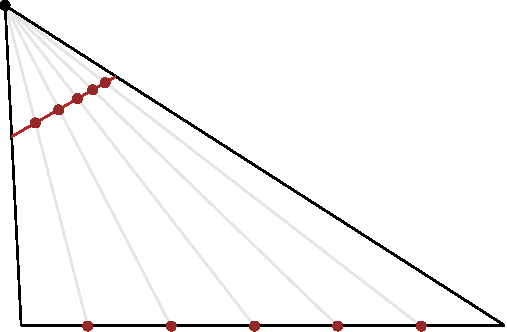
\includegraphics[scale=0.75]{figures/ProjectedGridVsWorldSpace.pdf}
\label{fig:subfigprojgrid1}
}
\subbottom[Increase]
{
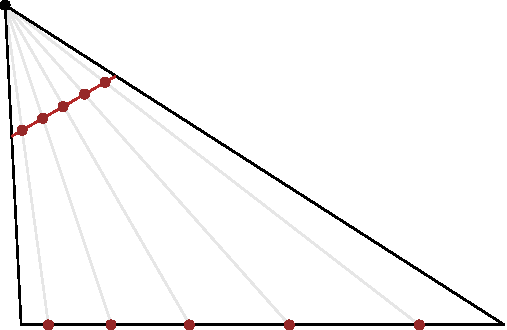
\includegraphics[scale=0.75]{figures/ProjectedGridUniform.pdf}
\label{fig:subfigprojgrid2}
}
\caption[The Projected Grid Concept]{The image on the left
~\subcaptionref{fig:subfigprojgrid1} shows an uniform grid in worldspace, it's
projection onto the image plane is not uniformly spaced though. The image on the
right~\subcaptionref{fig:subfigprojgrid2} on the other hand depicts an uniform grid on
the image plane and its associated non-uniform spaced worldspace positions.}
\label{fig:projectedgrid}
\end{figure}

% The algorithm used for the projected grid can be broken down into the following
% steps:
% \begin{itemize}
%  \item create a uniformly spaced grid orthogonal to the viewer using normalised
% device coordinates
%  \item transform the grid to worldspace
%  \item project the grid onto the desired base plane
%  \item apply height displacement
%  \item run the grid through the rendering pipeline as usual
% \end{itemize}

\newcommand{\mvec}[1]{\mathbf{#1}}
\newcommand{\mvecx}[1]{\mathbf{#1}_x}
\newcommand{\mvecy}[1]{\mathbf{#1}_y}
\newcommand{\mvecz}[1]{\mathbf{#1}_z}
\newcommand{\mvecw}[1]{\mathbf{#1}_w}
\newcommand{\mmat}[1]{\mathbf{#1}}

Let $\mvec{x}$ be a column vector representing the homogeneous world space
coordinate of a vertex, $\mmat{V}$ the view matrix and $\mmat{P}$ the
projection matrix, then
\begin{equation}
\label{eq:ws_to_cs}
 \mvec{c} = \mmat{P} \mmat{V} \mvec{x}
\end{equation}
where $\mvec{c}$ is the \textit{clip space} coordinate of $\mvec{x}$. For $\mvec{c}$ to
be inside the view frustum defined by $\mmat{P}$, $\mvec{c}$ is required to
meet the following condition
\begin{equation}
\label{eq:cs_bounds}
 \mvecx{c}, \mvecy{c}, \mvecz{c} \in \interval{-\mvecw{c}}{\mvecw{c}}
\end{equation}
where $\mvecw{c}$ is the homogeneous component of $\mvec{c}$. Next, clip space
vertex $\mvec{c}$ is transformed by the \textit{perspective division} as follows
\begin{equation}
\label{eq:cs_to_ndc}
 \mvec{n} = \frac{1}{\mvecw{c}}(\mvecx{c}, \mvecy{c}, \mvecz{c})^\mathsf{T}
\end{equation}
where $\mvec{n}$ corresponds to the \textit{normalised device coordinate},
\textit{NDC} in short, of $\mvec{c}$. As one can see, equations~\ref{eq:cs_bounds}
and~\ref{eq:cs_to_ndc} imply
\begin{equation}
\label{eq:ndc_bounds}
 \mvecx{n}, \mvecy{n}, \mvecz{n} \in \interval{-1}{1}
\end{equation}
which defines the space NDC reside in, namely the \textit{canonical view volume},
a three dimensional cube centered at the origin, with a side length equal two.\\


The projected grid, on the other hand, starts inside the canonical view volume
and needs to transform the vertices back to world space.

\begin{equation}
\label{eq:ndc_to_cs}
 \mvec{c} = (\mvecx{n}, \mvecy{n}, \mvecz{n}, 1)^\mathsf{T}
\end{equation}

\begin{equation}
\label{eq:cs_to_wsh}
 \mvec{w} = (\mmat{P} \mmat{V})^\mathsf{-1} \mvec{c}
\end{equation}

\begin{equation}
\label{eq:wsh_to_ws}
 \mvec{x} = \frac{1}{\mvecw{w}}(\mvecx{w}, \mvecy{w}, \mvecz{w}, \mvecw{w})^\mathsf{T}
\end{equation}

To simplify matters the grid may be consist of vertices defined by
two-dimensional normalised device coordinates. In order to project the grid
onto a plane a ray has to be setup for every vertex.

postprojection coordinates transformed to worldspace
grid on near and far plane, intersection with the y=0 plane
decouple projector from camera
